\documentclass{standalone}
\usepackage{tikz}
\usepackage{ctex,siunitx}
\setCJKmainfont{Noto Serif CJK SC}
\usepackage{tkz-euclide}
\usepackage{amsmath}
\usetikzlibrary{patterns, calc,3d}
\usetikzlibrary {decorations.pathmorphing,decorations.pathreplacing,decorations.shapes}
\tikzset{label style/.append style={font=\small}}
\begin{document}
\small
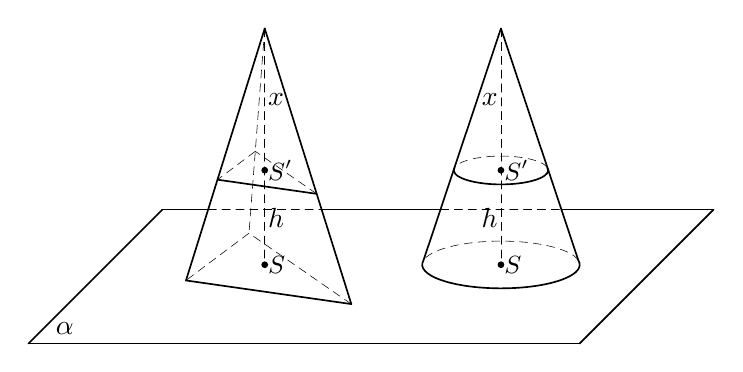
\begin{tikzpicture}[>=latex,scale=1.0,inner sep=1pt]
  \tkzDefPoints{0/0/C,7/0/D,8.7/1.7/E,1.7/1.7/F}
  \tkzDefPoints{6/1/O,6/4/H,4/1/R}
  \tkzDefPoints{3/1/O',3/4/H',2/0.8/M,4.1/0.5/N,2.8/1.4/Q}
  \tkzDefShiftPoint[O]({cos(10)},{0.3*sin(10)}){rr}
  \tkzDefShiftPoint[O]({cos(170)},{0.3*sin(170)}){rl}
  \tkzDefPointOnLine[pos=0.6](H,rr)\tkzGetPoint{rr'}
  \tkzDefPointOnLine[pos=0.6](H,rl)\tkzGetPoint{rl'}
  \tkzDefPointOnLine[pos=0.6](H,O)\tkzGetPoint{O1}
  \tkzDefPointOnLine[pos=0.6](H',O')\tkzGetPoint{O2}
  \tkzDefPointOnLine[pos=0.6](H',M)\tkzGetPoint{M'}
  \tkzDefPointOnLine[pos=0.6](H',N)\tkzGetPoint{N'}
  \tkzDefPointOnLine[pos=0.6](H',Q)\tkzGetPoint{Q'}
  \tkzInterLL(E,F)(H,rl)\tkzGetPoint{LL}
  \tkzInterLL(E,F)(H,rr)\tkzGetPoint{LR}
  \tkzInterLL(E,F)(H',M)\tkzGetPoint{Ll}
  \tkzInterLL(E,F)(H',N)\tkzGetPoint{Lr}
  \tkzDrawSegments[densely dashed](H,O H',Q Q,M N,Q H',O' N',Q' Q',M' Ll,Lr LL,LR)
  \tkzDrawPoints[fill=black](O,O1,O',O2)
  \tkzDrawSegments[semithick](F,C C,D D,E H,rr H,rl M,N H',M H',N M',N' Lr,LL LR,E F,Ll)
  \draw[semithick](rr)arc(10:-190:1 and 0.3);
  \draw[very thin,densely dashed](rr)arc(10:170:1 and 0.3);
  \draw[semithick](rr')arc(10:-190:0.6 and 0.18);
  \draw[very thin,densely dashed](rr')arc(10:170:0.6 and 0.18);
  \tkzLabelLine[pos=0.5,left](O,O1){$h$}
  \tkzLabelLine[pos=0.5,left](O1,H){$x$}
  \tkzLabelLine[pos=0.5,right](O',O2){$h$}
  \tkzLabelLine[pos=0.5,right](O2,H'){$x$}
  \tkzLabelPoint[right](O){$S$}
  \tkzLabelPoint[right](O1){$S'$}
  \tkzLabelPoint[right](O'){$S$}
  \tkzLabelPoint[right](O2){$S'$}
  \tkzLabelAngle[pos=0.5](D,C,F){$\alpha$}
\end{tikzpicture}
\end{document}